\documentclass{article}
\usepackage[utf8]{inputenc}
\usepackage{graphicx}


\graphicspath{ {/home/nooremf/Project/Code/Thesis/}}
\newcommand*{\1}{\hspace{1pt}}
\title{Comparison Between The Classical and Quantum Properties of Ideal Gas.}

\author{ COURSE CODE : TP-407 \\ \textbf{SUBMITTED BY}
 \\  CLASS ROLL : SK-098-034 \  EXAM ROLL: 30222 \\
 REGISTRATION NUMBER : 2016-714-720 \\     SESSION : 2016-17
\\ 
\includegraphics[width=0.3\textheight]{DU.jpg} \\  DEPARTMENT OF THEORETICAL PHYSICS \\ UNIVERSITY OF DHAKA 
}
\date{March 2022}

\begin{document}

\maketitle
\newpage
\tableofcontents
\listoffigures

\newpage
\section*{Abstract}
    There are so many studies on the difference between classical and quantum properties still there are so many scopes to do study on this topic. In this paper, it 
    has been shown about thermodynamic properties of classical and quantum to observe their difference. The thermodynamics properties such as specific heat, internal energy
    free energy, entropy, have been examined here to compare the properties. About specific heat we got that classical result doesn't match with experimental value.
    But quantum meachinal result has a good agreement with experiment which is derived from Debye. We also examined theoretically the Gibbs paradox for both classical
    and quantum gas.   
\newpage
\section{Introduction}
Our goal is to compare classical and quantum properties of ideal gas. Here we took the help of statistical mechanics. Statistical mechanics is a formulae which aims to explain physical properties of matter. It has been applied to the study of matter in the solid state,liquid state or gaseous state. We will discuss about gaseous state.\\



The history of statistical mechanics is interwined with that of thermodynamics and kinetic energy.  Thermodynamics deduces relations independent of the properties of molecules and mechanisms of their interactions.\\


The basic ideas were developed mainly during the second half of nineteenth century .However we shall start our story with the work of Daniel Bernoulli in 1738. He assumed that the pressure of a gas was due to the impacts of the gas particles on the enclosure walls and he succeeded in deducing Boyel's law.\\


In 1857, Clausias derived the ideal gas law.

After that, in 1859 ,Clerk Clausias and Maxwell published their first paper on molecular velocities. It is the famous \textbf{Maxwell Distribution}\cite{l3} of molecular velocities of gas in equilibrium state.\\




By that time,Boltzman had already made his first strides.In 1868-71, he extended Maxwell's theory and showed that with every degree of freedom of a gas molecule there is associated the same mean energy. Boltzman's great contribution was to give the relation between entropy and probability and the famous equation S=klnW. This work laid the formulation of what we call now\textbf{Classical} or \textbf{Maxwell-Boltzman statistics}\cite{l3}.\\



In 1873, Van der Wa'als proposed his famous equation of state, which allows qualitatively both for the finite size of the molecules and their mutual attraction.\\




At the turn of 20th century, with the advent of quantum hypothesis, Plank used statistical method to treat black-body radiation as a photon gas.

In 1907, this method was followed by Einstein's work on the heat capacity of solid\cite{l1}, this was later modifies by Debye.\\


In 1924, a great advantage was made when the combination of quantum and statistical ideas lead to treatment of photon gas by \textbf{Bose-Einstein}\cite{l2} statistics.\\




Following the enunciation of Pauli's exclusion principle(1925), in 1926, Fermi showed that certain physical would obey different kind of statistics. That is called \textbf{Fermi-Dirac}\cite{l4} statistics,in which not more than one particle could occupy the same energy state.\\


It was shown that the Maxwell Boltzman distribution was the limiting case, at high temperature of Bose-Einstein and Fermi-Dirac distribution.\cite{l4}\\



In 1940, the unusual properties of liquid $4He$ and $3He$, we explained by treating them as Bose-Einstein and Fermi-Dirac studies respectively.\\


Apart from the forgoing milestones, several notable contribution towards the development of statistical mechanics have been made from time to time.\\


However most of these contributions are concerned with the development or perfection of physical problems more fruitful.\\

The purpose of this paper is to study some problems of statistical physics based on classical and quantum mechanics and to derive the thermodynamics quantities in different statistics ensembles for some physical system. According to properties ideal gas can be divided into 2 gas particle.One is classical ideal gas,that follows Maxwell-Boltzman distribution.Another one is quantum ideal gas, that follows Bose-Einstein statistics and Fermi-Dirac statistics.Gas, which follows Bose-Einstein  statistics, is called ideal Bose gas and which follows Fermi-Dirac statistics, is called ideal Fermi gas.
To determine the properties of these gas, we use statistical mechanics.This method enables us to predict the properties of matter. In other word,the are a 'bridge' which take us from microscopic description of matter to macroscopic thermodynamics description.\\

This latter description of substance involves parameter such as internal energy, specific heat(heat capacity), entropy etc and such quantities can be derived from model describing molecular or microscopic behaviour of substance. At the first stage we have derived classical properties and we have studied the Fermi and BoseOf ideal gas properties. Each section propetries such as entropy, free energy, Helmholtz energy, internal energy, specific heat etc have been derived. \\ 
We also studied about some properties solid state such as Einstein's model specific, and Debye model of specific heat.
\newpage

\subsection{Classical Properties of Ideal Gas}
\subsubsection{thermodynamic properties}
\begin{itemize}
\item \textbf{specific heat}
    
\end{itemize}
First law of thermodynamics:\\ 
\begin{equation}
dQ=dE+PdV
\end{equation}

If volume is constant ,V=0;\\

Specific heat\cite{l5}\\


   $  C_v  = \left(\frac{dQ}{dT}\right)_V $\\
    $    C_v =\frac{3}{2}R$\\
\begin{figure}[htb!]
    \centering
    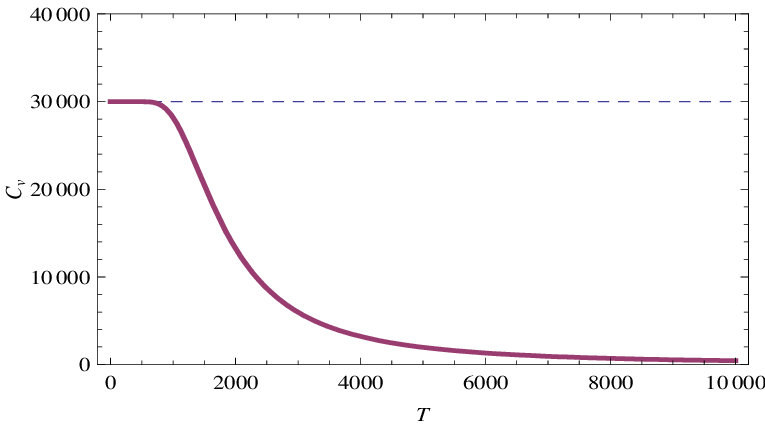
\includegraphics[scale=0.3]{Cv}
    \caption{Specific heat of classical gas}
    \label{fig:my_label}
\end{figure}

which is temperature independent

\begin{itemize}
    \item \textbf{Internal Energy}
\end{itemize}

classically,Internal Energy\cite{l6} 
\begin{equation}
    U=\frac{3}{2}RT
\end{equation}
\subsection{\textbf{Partition Function}}

Partition function of classical gas is,
\begin{equation}
  Z=\frac{v}{h^3}(2\pi mkT)^{\frac{3}{2}}  
\end{equation}
For N particle 
\begin{equation}
    Z=[\frac{V}{h^3}(2\pi mkT)^{\frac{3}{2}}]^N
\end{equation}
By using partition function we can derive free energy,internal energy,entropy etc\cite{l6}.
\begin{itemize}
    \item \textbf{Free Energy}
\end{itemize}
Here\\

Volume=V\\

Internal energy=U\\

The number of particles=N\\

Free energy,\\


 $ F=-kTlnZ$ \\
 
     =$-kT[{\frac{V}{h^3}}(2\pi  mkT)^{\frac{3}{2}}]^N$ \\
     
     =$-NkTln[\frac{v}{h^3}(2\pi mkT)^{\frac{3}{2}}]$\\
     
     
 


\begin{itemize}
    \item \textbf{Internal Energy}
\end{itemize}

Internal energy of classical gas,\\


   $U=NkT^2\frac{dlnZ}{dT}$\\

   $=RT^2\frac{dlnZ}{dT}$\\
   
   
\begin{itemize}
    \item\textbf{Entropy} \cite{l8} 
\end{itemize}
We know,$F=U-TS$\
\
So,$dF=dU-TdS-SdT$\\

and $dQ=dU+PdV-\mu dN$\\

    $TdS=dU+PdV-\mu dN$\\
    
\ $dU=TdS-PdV+\mu dN$\\

Now,\\
$dF=TdS-PdV+\mu dN-TdS-SdT$\\

$dF=PdV+\mu dN-SdT$\\

But\\
\\
V,N is constant\\

$dF=-SdT$\\

$S=-\frac{dF}{dT}$\\

Entropy,\\ 
\\
$S=-\frac{dF}{dT}$\\

     $=Nkln[\frac{V}{h^3}(2\pi mkT)^{\frac{3}{2}}]+\frac{T.T^{\frac{1}{2}}}{T^{\frac{3}{2}}}\frac{3}{2}]$\\
     
     $=Nkln[\frac{V}{h^3}(2\pi mkT)^{\frac{3}{2}}+\frac{3}{2}]$\\

     From this equation, we see that at temperature T $\rightarrow$ 0, entropy S = $Nkln \ 3/2$ 

     But accordingly, third law of thermodynamics T $\rightarrow$ 0, S  $\rightarrow$ 0. That does not satisfy Third law of thermodymics.
     
     \begin{figure}
    \centering
    \includegraphics[scale=2]{entropy}
    \caption{Entropy of classical gas}
    \label{fig:my_label}
\end{figure}

     \begin{itemize}
    \item \textbf{Gibbs Paradox} \cite{l9}
\end{itemize}

We know,\\


Entropy,$S =Nkln[\frac{V}{h^3}(2\pi mkT)^{\frac{3}{2}}+\frac{3}{2}]$\\
    


By mixing two entropy at constant T and pressure P,\\

Let,\\

$E=2E$\\

$N=2N$\\

$V=2V$\\
\\
With constant temperature T and P\\
It should be $S = 2S$ but there is paradox 2kln \ 2.
Then\\

Entropy,$S=Nkln[\frac{V}{h^3}(2\pi mkT)^{\frac{3}{2}}+\frac{3}{2}]$\\

$ =  2Nkln[\frac{2V}{h^3}(2\pi mkT)^{\frac{3}{2}}+\frac{3}{2}]$\\

$ =2Nkln2+2Nkln[\frac{V}{h^3}(2\pi mkT)^{\frac{3}{2}}+\frac{3}{2}]$\\


$S= 2S+2Nkln2$\\


    
    






     
\begin{itemize}
    \item \textbf{State equation}
\end{itemize}     

The pessure of the system is\\

$P=\frac{NKT}{V}$\\





\section{Quantum properties of ideal gas}

At first we derive specific heat of ideal gas by quantum mechanics:\\
\subsubsection{Einstein model of specific heat}

\begin{itemize}
    \item Assumptions
\end{itemize}
\textbf{1.} Atoms are vibrating about their equilibrium position.\\

\textbf{2.}All atoms are independent having some vibration frequency.\\

\textbf{3.} An atom can be considered as harmonic oscillator and one atom is equivalent to three harmonic oscillator.\\

The energy of harmonic oscillator is\\

$E_n=(n+\frac{1}{2})$\\

Therefore,the energy of harmonic oscillator,\\

 $E=\sum E_n e^{-\frac{E_n}{kT}}$\\
 
 Total energy,
 $E=\frac{h\nu}{e^{\frac{h\nu}{kT}}-1}$\\

Energy for 1 mole of solid,\\

$E=3N_A(\frac{h\nu}{e^{\frac{h\nu}{kT}}-1})$\\

Specific heat:\\

$C_v=(\frac{dE}{dT})_v$\\

 $ =3N_A(\frac{h\nu}{kT})^2$
 ${e^{\frac{h\nu}{kT}}}$
$(\frac{1}{e^{\frac{h\nu}{kT}}-1})^2$\\

let,\\

$\frac{h\nu}{k}=\theta$\\

Now,\\

    $C_v=3R(\frac{\theta_E}{T})^2{e^{\frac{\theta_E}{T}}} $
    $(\frac{1}{e^{\frac{\theta_E}{T}-1}})^2$\\
    
This is the expression for $C_v$ according to Einstein model.\\


\begin{figure}[h!]
    \centering
    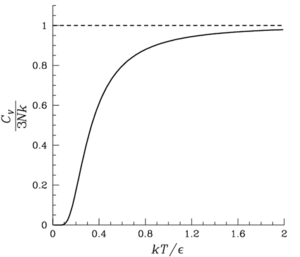
\includegraphics[scale=0.7]{cv for einstein}
    \caption{Specific heat of Einstein model}
    \label{fig:my_label}
\end{figure}

\subsubsection{\textbf{Debye theory of specific heat}}

In the year 1912,Peter Debye\cite{l10} has given a new model on specific heat on solid with following assumption\\

\textbf{1.}  Atoms are not vibrating independently. Due to inter atomic interactions the motion or vibration of one atom may have a significance effect on its nearest. This is to be continued to the whole whole crystal to get lattice vibration.\\

\textbf{2.} The solid is not vibrating with a single frequency $\nu$, it can vibrate in many different ways with many different frequency.\\

In Debye theory, solid is regarded as phonon gas.\\

Let,\\

n=positive integer corresponds to individual frequency.\\

$n=\frac{2L\nu}{v}$\\

v=velocity of sound wave.\\

n corresponds to $\nu$,$n+dn$ corresponds to $\nu+d\nu$.\\

Volume for shell $ n+dn$ is $4\pi n^2dn$ and ($\frac{1}{8} 4\pi n^2 dn$) corresponds to positive n.\\

So,\\

$g(\nu)d\nu=\frac{1}{8}4\pi n^2 dn$\\

$=4\pi v(\frac{1}{v^3})\nu^2d\nu$  [substitute the value of n]\\


Here,\\

$\frac{1}{v^3}=\frac{1}{v_L^3}+\frac{2}{v_t^3}$\\


$v_L$=velocity corresponding to longitudinal mode of vibration.\\

$v_t$=velocity corresponding to transeverse mode of vibration.\\

Now we can write,\\

$\int_v g(\nu)d\nu=3N$\\


$=>4\pi V(\frac{1}{v_L^3}+\frac{2}{v_t^3})\frac{\nu_D^3}{3}=3N$\\

$=>4\pi V(\frac{1}{v_L^3}+\frac{2}{v_t^3})=\frac{9N}{\nu_D^3}$\\

The average energy,\\

    $<E>=\frac{h\nu}{e^{\frac{h\nu}{kT}}-1}$\\
    
Total energy \\

$E=3N<E>$\\

$=\int g(\nu)d\nu \frac{h\nu}{e^{\frac{h\nu}{kT}}-1}$\\


$E=\frac{9N}{\nu_D^3}\int\frac{h\nu^3}{e^{\frac{h\nu}{kT}}-1}$\\

Let,\\

$x=\frac{h\nu}{kT} $\\

Now,\\

$E=\frac{9N(kT)^4}{\nu_D^3h^3}\int\frac{x^3}{e^x-1}dx$\\

Again,\\

let,\\

$\theta_D=\frac{h\nu_D}{k}$\\




$E=9N(\frac{T}{\theta_D})^3\int\frac{x^3}{e^x-1}dx$\\


Expression of energy in Debye model.\\

For,\textbf{higher temperature}\\

$T>>\theta_D$\\

$E=3NkT$\\

So ,specific heat becomes ,\\

$C_v=3NK$\\

  $ =3R$\\
  
For,\textbf{lower temperature}\\

$T<<\theta_D$\\

$E=\frac{3}{5}\frac{\pi^4RT^4}{\theta_D^3}$\\


Specific heat becomes,\\
\begin{figure}
    \centering
    \includegraphics[scale=0.8]{300px-DebyeVSEinstein}
    \caption{Specific heat Debye vs Einstein}
    \label{fig:my_label}
\end{figure}
$C_vfigure=(\frac{dE}{dT})_v$\\


 $ = \frac{12\pi^4R}{5\theta_D^3}T^3$\\
 
 So,at lower temperature specific heat is proportinal to $T^3$.\\
 
 \begin{itemize}
     \item \textbf{Gibbs paradox}
 \end{itemize}
 
 As quantum particle indistinguishable,\\
 
 The entropy is,$S=Nkln[\frac{V}{h^3}(2\pi mkT)^{\frac{3}{2}}+\frac{5}{2}]$\\
 
 By mixing entropy at constant temperature T,pressure P.\\
 
 Let\\
 
 $N=2N$\\
 
 $V=2V$\\
 
 $E=2E$\\
 
 $S=Nkln[\frac{V}{Nh^3}(2\pi mkT)^{\frac{3}{2}}+\frac{5}{2}]$\\
 
 $= 2Nkln[\frac{2V}{2Nh^3}(2\pi mkT)^{\frac{3}{2}}+\frac{5}{2}]$\\
 
 $=   2Nkln[\frac{V}{Nh^3}(2\pi mkT)^{\frac{3}{2}}+\frac{5}{2}]$\\
 
 $S=2S$\\
 Though there is no paradox, but at T$\rightarrow$ 0 S $=$ 2Nkln \ 5/2
 It also doesn't satisfy third law of thermodynamics.  
 
\subsection{\textbf{Thermodynamics properties of ideal Fermi gas}} 

For the case of Fermi gas,the energy level cannot be occupied by more than one particle(fermion).\\

Grand Partition function for Fermi gas:\\

$Z(z,v,T)=\sum\frac{1}{1-ze^{-\beta}E}$\\

Now,\\

$\frac{PV}{kT}=lnZ ...  ...  ...  ..........(1)$\\

and\\

The mean number of the Fermions is\\

$N=\sum(<n_E>)=\sum\frac{1}{z^-1e^(\beta E)+1}............................(2)$\\

Here,\\

$\beta=\frac{1}{kT}$\\

and\\

$z=e^{\frac{\mu}{kT}}$\\

If we replace summation over E by corresponding integration , equation 1 and equation 2 becomes\\

$\frac{p}{kT}=\frac{g}{\lambda^3}f_\frac{5}{2}(z)$\\

$\frac{N}{V}=\frac{g}{\lambda^3}f_\frac{3}{2}(z)$\\

$\lambda =\frac{h}{(2\pi mkT)^{\frac{3}{2}}}$\\

$f_\mu(z)$ is Fermi function.\\


\begin{itemize}
    \item \textbf{Internal Energy}
\end{itemize}

The internal energy of Fermi gas\\

$U=-(\frac{dlnZ}{d \beta})$\\

$ =kT^2(\frac{dlnZ}{dT})$\\

$ = \frac{3}{2}kT\frac{gV}{\lambda^3}f_\frac{5}{2}(z)$\\

$ =\frac{3}{2}NkT\frac{f_\frac{5}{2}(z)}{f_\frac{3}{2}(z)}$\\

\begin{itemize}
    \item \textbf{Pressure}
\end{itemize}


Pressure for Fermi Gas is,\\

$P=\frac{2}{3}\frac{U}{V}$\\
\newpage
\begin{itemize}
    \item \textbf{Helmholtz free energy}
\end{itemize}

For the Helmholtz free energy of a gas\\

$A=N\mu-PV$\\

$ =NkT[{lnz-\frac{f_\frac{5}{2}(z)}{f_\frac{3}{2}(z)}}]$\\


\begin{itemize}
    \item \textbf{Entropy}
\end{itemize}

Entropy for Fermi gas\\

$S=\frac{U-A}{T}$\\

$ =NkT[\frac{5}{2}\frac{f_\frac{5}{2}(z)}{f_\frac{3}{2}(z)}-lnz]$\\

\begin{itemize}
    \item \textbf{Specific heat}
\end{itemize}

The specific heat of Fermi gas\\

$  C_v=(\frac{dU}{dT})$\\

$C_v=Nk[\frac{15}{4}\frac{f_\frac{5}{2}(z)}{f_\frac{3}{2}(z)}-\frac{9}{4}\frac{f_\frac{5}{2}(z)}{f_\frac{3}{2}(z)}]$\\
\begin{figure}[htb!]
    \centering
    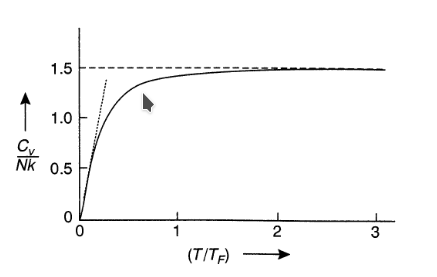
\includegraphics[scale=0.5]{lamia3}
    \caption{The specific heat of an ideal Fermi gas the dotted line depicts the linear behaviour at low temperature }
    \label{fig:my_label}
\end{figure}


\subsection{Thermodynamics properties of ideal Bose gas }

We will now consider N particles with zero spin (bosons) without interaction, enclosed in a volume V. We assume that the system is in thermodynamical equilibrium in temperature T. We will study some properties of the ideal gas of bosons.\\

Grand partition function for Bose gas\\

$Z(z,v,T)=\sum(1+ze^{\beta E})$\\

\begin{itemize}
    \item \textbf{State equation}
\end{itemize}

$\frac{PV}{kT}=lnZ$...................(3)\\

$N=\sum<n_E>$\\

$ = \sum\frac{1}{z^{-1}e^{\beta E}}$\\

By integrating both of them instead of summation\\

$\frac{P}{kT}=\frac{1}{\lambda^3}g_\frac{5}{2}(z)-\frac{1}{V}ln(1-z)$\\

$\frac{N}{V}=\frac{1}{\lambda^3}g_\frac{3}{2}(z)+\frac{1}{V}\frac{z}{1-z}$\\

Here,$\lambda=\frac{h}{(2\pi mkT)^{\frac{3}{2}}}$ is mean free path\\

Here,$g_\mu(z) is Bose function $

If z<1,then following two equation becomes \\

$\frac{P}{kT}=\frac{1}{\lambda^3}g_\frac{5}{2}(z)$\\

$\frac{N}{V}=\frac{1}{\lambda^3}(z)$
\begin{itemize}
    \item \textbf{Internal Energy}
\end{itemize}

The internal energy of Bose gas,\\

$U=-(\frac{dlnz}{d\beta})$\\

$ = kT^2[\frac{d}{dT}(\frac{PV}{kT})]$\\

$ = \frac{3}{2}kT\frac{V}{\lambda^3}g_\frac{5}{2}(z)$\\

\begin{itemize}
    \item \textbf{Pressure}
\end{itemize}

Pressure for Bose gas,\\

$P=\frac{N}{V}kT\frac{g_\frac{5}{2}(z)}{g_\frac{3}{2}(z)}$\\


\begin{itemize}
    \item \textbf{Specific heat }
\end{itemize}

Specific heat of Bose gas,\\


$C_v=(\frac{dU}{dT})_v$\\

$ = Nk[\frac{d}{dT}(\frac{3}{2}T\frac{g_\frac{5}{2}(z)}{g_\frac{3}{2}(z)})]$\\

$ =\frac{15}{4}\frac{g_\frac{5}{2}(z)}{g_\frac{3}{2}(z)}-\frac{9}{4}\frac{g_\frac{3}{2}(z)}{g_\frac{1}{2}(z)} $\\

\begin{figure}[htb!]
    \centering
    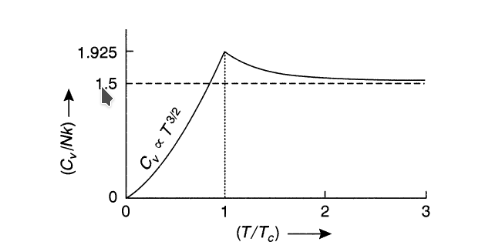
\includegraphics[scale=0.7]{lamia2}
    \caption{The specific heat of an ideal Bose gas as a function of the temperature parameter $\frac{T}{T_c}$}
    \label{fig:my_label}
\end{figure}
\begin{itemize}
    \item \textbf{Helmholtz free energy}
\end{itemize}

The Helmholtz energy for bose gas,\\

$A=N\mu-PV$\\

$ = NkT(lnz-V\frac{g_\frac{5}{2}(z)}{N\lambda^3})$\\


\begin{itemize}
    \item \textbf{Entropy}
\end{itemize}

we know,\\

$U-TS+PV=N\mu$\\


$ TS=U+PV-N\mu$\\

$S=\frac{U+PV-N\mu}{T}$\\

By substituting the value that obtained before\\


$ S =Nk(\frac{5}{2}\frac{g_\frac{5}{2}(z)}{g_\frac{3}{2}(z)}-lnz )$\\

\newpage
\begin{figure}[htb!]
    \centering
    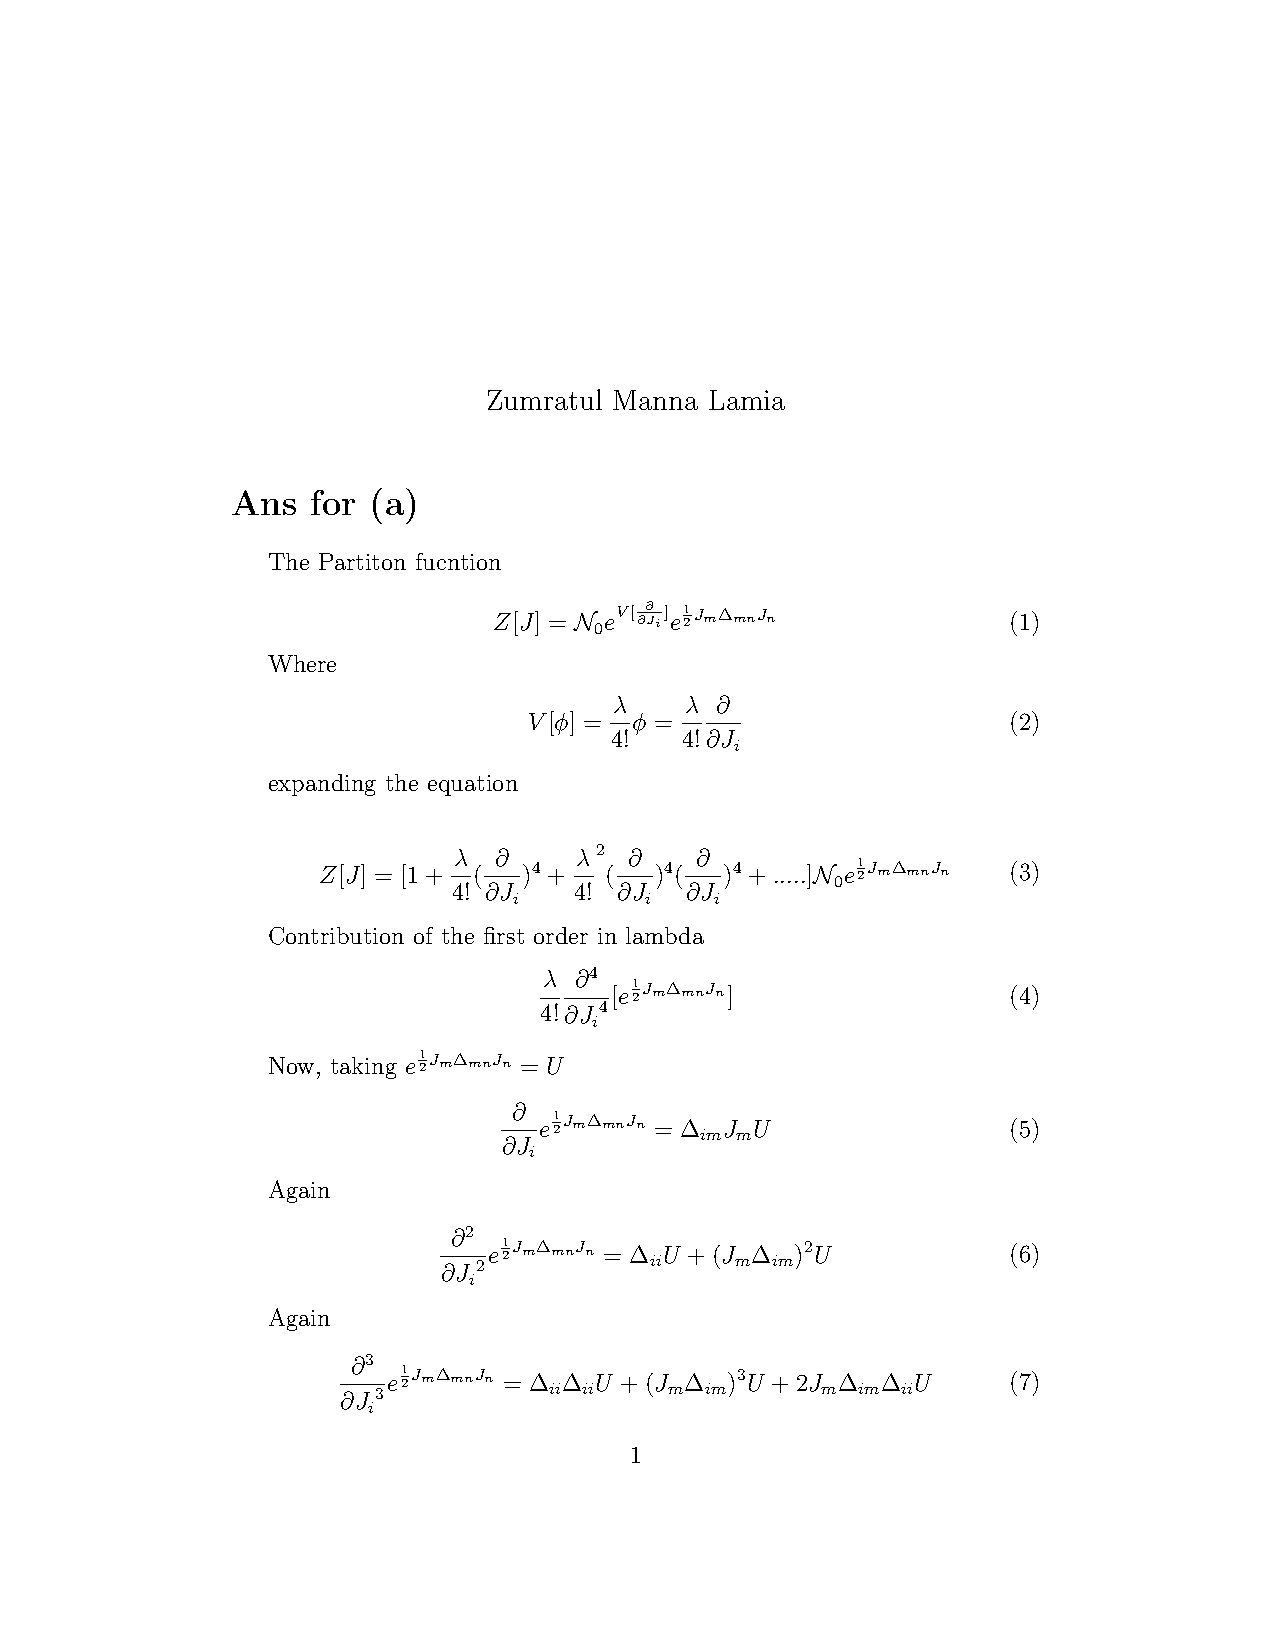
\includegraphics[scale=0.7]{lamia}
    \caption{Entropy for Fermi and Bose gas}
    \label{fig:my_label}
\end{figure}

\newpage

\subsection{Summary}

In this work, we have studied about some thermodynamical properties of ideal gas based on classical and quantum mechanics. We have found that, there are some difference between the properties of classical and quantum gas. We have derived specific heat classically, 3R which is temperature dependent. But experimentally specific heat is a function of T.This is the failure for classical theory to explain $C_v$. We have derived Einstein specific heat, but this is valid for only higher temperature.At lower temperature specific heat varies exponentially whereas specific heat varies $T^3$ experimentally.After that,at subsection Debye theory,it shows us that at higher and lower temperature $C_v$ is experimentally exact as theory. This is the success of Quantum theory .\\

Another success is there is no paradox in quantum theory . After mixing two individual entropy at temperature T,entropy should be $2S$. we have seen that entropy is $2S+2Nkln2$. Classically there always exists paradox. Quantum mechanically this is exact to SS after mixing individual entropy. 
But at  the entropy is 2S. This satisfy the Gibbs paradox. This is another success of quantum theory. \\ 
\\ 
Classically when we calculate entropy, it doesn't follow third law of thermodynamics. But in Quantum theory entropy satisfies third law of thermodymmics. It is anohter success of quantum theory


\newpage
\bibliographystyle{unsrt}
\bibliographystyle{plain}
\bibliography{main.bib}

\end{document}
